\documentclass[a4j]{ujarticle}
\usepackage[dvipdfmx]{graphicx}
\usepackage{url}
\usepackage{bbding}
\usepackage{lscape}
\usepackage[subrefformat=parens]{subcaption}
\usepackage{bm}
\usepackage{amsmath}

\title{ミーティング資料}
\author{安達智哉\\to-adachi@ist.osaka-u.ac.jp}
\date{2019年5月9日}

\begin{document}
\maketitle

\section{メモリ負荷の算出}
文献\cite{3gpp.23.720}に示されているコネクション確立に伴うシグナリング図を図\ref{Legacy_connection_setup}に示す。
UEがIdle状態からConnected状態へ遷移する際に発生しているシグナリングを調査することにより、各ノードのメモリが保持する情報を推定することができる。
今回はMMEが関与しているシグナリングについてOAIのソースコードを元に調査を行った。
OAIのソースコード(OpenairinterfaceCN-develop)では、各シグナリングに含まれる情報が構造体として定義されていた。
それらの構造体に含まれるメンバのバイト数を足し合わせることによりシグナリングメッセージに含まれる情報量を知ることができる。

\begin{figure}[htbp]
  \centering
  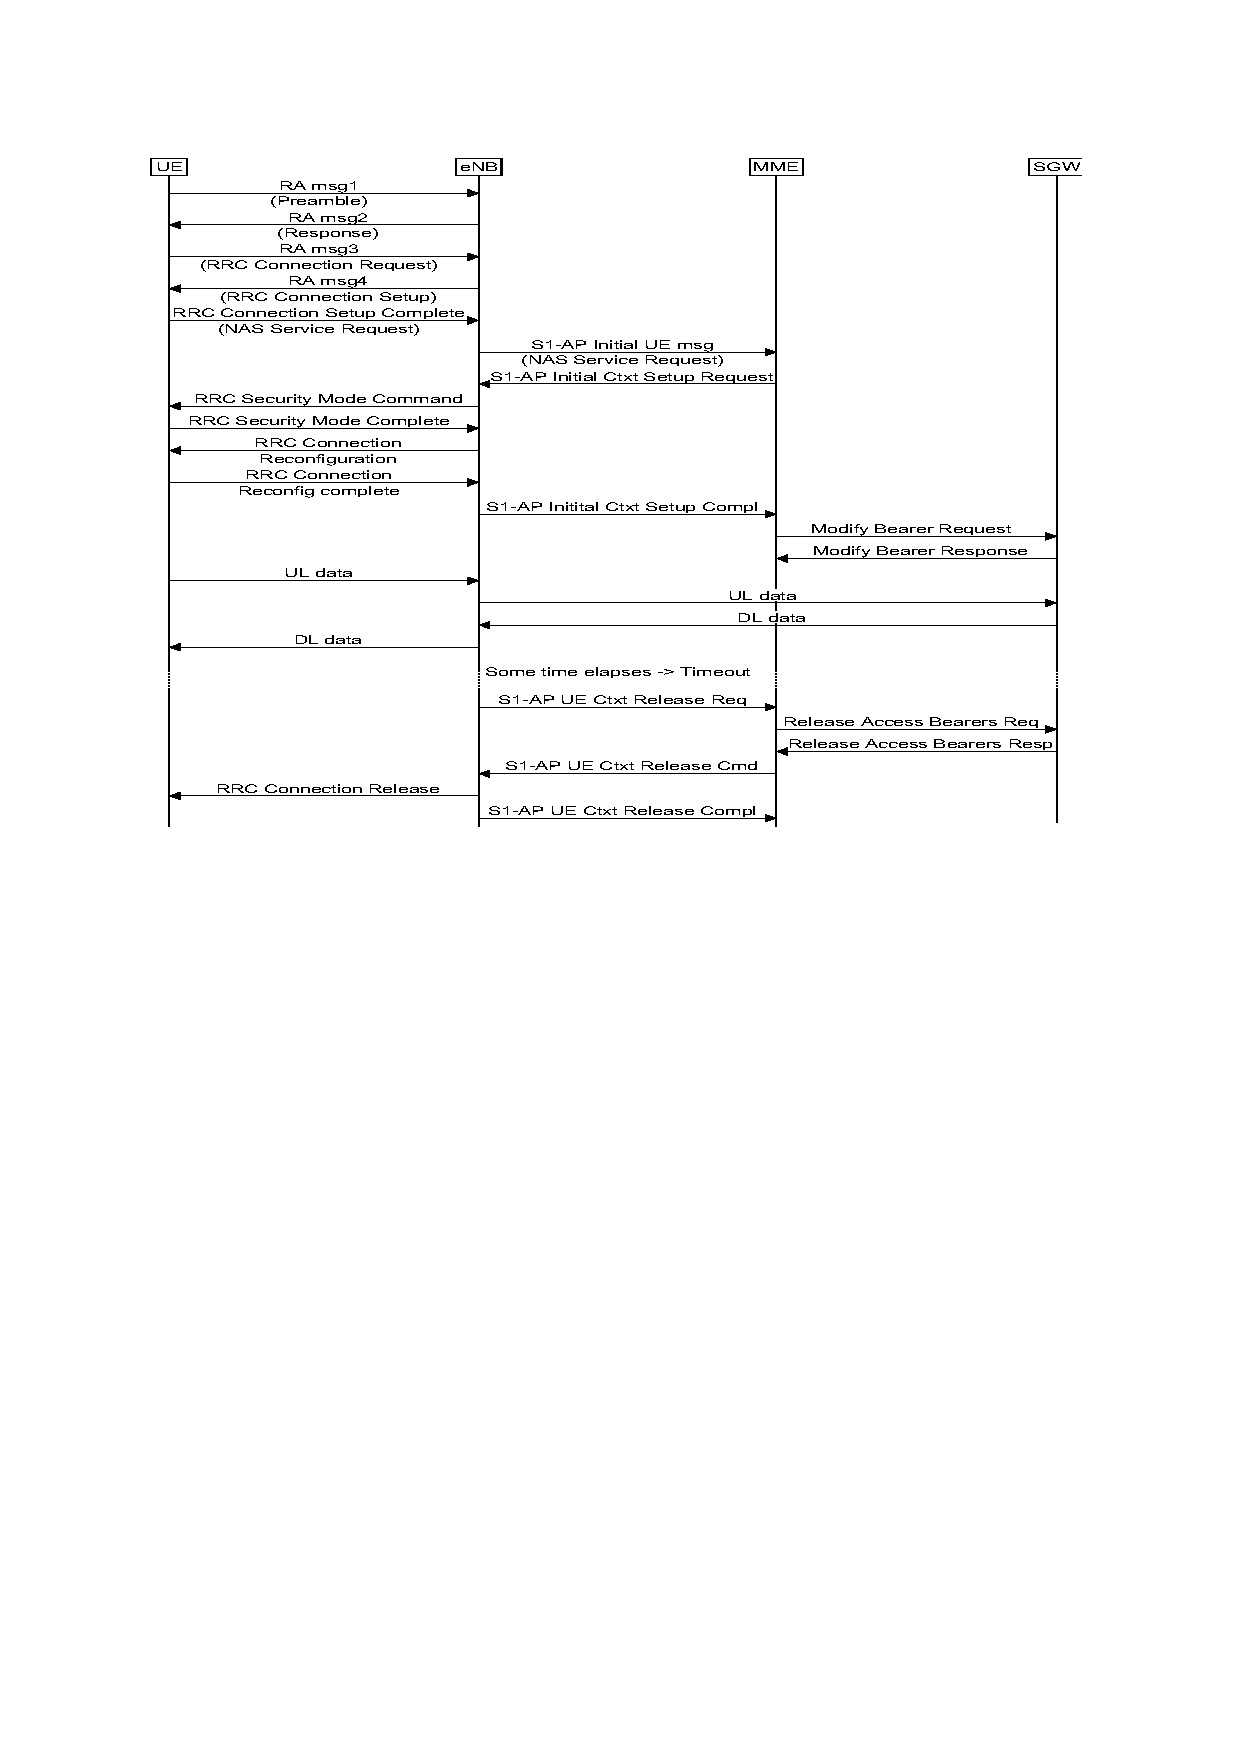
\includegraphics[width=0.9\hsize]{Legacy_connection_setup.pdf}
  \caption{Legacy connection setup}
  \label{Legacy_connection_setup}
\end{figure}


各シグナリングメッセージに含まれる情報量を調査した。
調査結果を以下の表\ref{table:oai_signal_memory}に示す。
\begin{table}[htbp]
  \centering
  \caption{各シグナリングの情報量(OAIベース)}
  \label{table:oai_signal_memory}
  \begin{tabular}{l|l|l}
    \hline
    シグナリング  & OAIで定義されている構造体 & 情報量(bit)  \\ \hline \hline
    S1-AP Initial UE msg  & \verb|itti_s1ap_initial_ue_message_s| & 140\\
    S1-AP Initial Ctxt Setup Request  & \verb|itti_s1ap_initial_ctxt_setup_req_s| & 908\\
    S1-AP Initital Ctxt Setup Compl & (not found)  &  -\\
    Modify Bearer Request & \verb|itti_s11_modify_bearer_request_s|  &  7726\\
    Modify Bearer Response  & \verb|itti_s11_modify_bearer_response_s| &  392\\
    S1-AP UE Ctxt Release Req & \verb|itti_s1ap_ue_context_release_req_s|  &  88\\
    Release Access Bearers Req  & \verb|itti_s11_release_access_bearers_request_s| &  208\\
    Release Access Bearers Resp & \verb|itti_s11_release_access_bearers_response_s| & 392\\
    S1-AP UE Ctxt Release Cmd  & \verb|itti_s1ap_ue_context_release_command_s| &  112\\
    S1-AP UE Ctxt Release Compl  & \verb|itti_s1ap_ue_context_release_complete_s|  &  56\\\hline
  \end{tabular}
\end{table}
表\ref{table:oai_signal_memory}を見ると、シグナリングによって含まれている情報量が大きく異なることが分かる。
特にModify Bearer Requestに含まれる情報は7726 bitであり、他のシグナリングと比較して最も大きいことが分かった。
また、S1-AP Initital Ctxt Setup Complに関するコードをOAIのソースコードには見つけることができなかった。
OAIではこのシグナリングを実装していないかもしくは別名のシグナリングとして実装している可能性がある。

各シグナリングに含まれる主な情報を以下の表\ref{table:oai_signal_content}に示す。
\begin{table}[htbp]
  \centering
  \caption{各シグナリングに含まれる(OAIベース)}
  \label{table:oai_signal_content}
  \begin{tabular}{c|l}
    \hline
    構造体  & 含まれている主要な情報  \\ \hline \hline
    & eNB UE S1AP ID\\
    S1-AP Initial UE msg& MME UE S1AP ID\\
    & The E-UTRAN Cell Global Identification (ECGI)\\\hline
    & eNB UE S1AP ID\\
    & MME UE S1AP ID\\
    & Key eNB \\
    S1-AP Initial Ctxt Setup Request  & EPS bearer ID \\
    & QoS情報 \\
    & S-GW TEID for user-plan \\
    & S-GW IP address for User-Plane \\\hline
    S1-AP Initital Ctxt Setup Compl & -\\\hline
    & TEID\\
    & ME Identity (MEI)\\
    Modify Bearer Request & Delay Value\\
    & bearer context to be modified\\
    & UE Time Zone\\\hline
    & TEID\\
    & linked eps bearer id\\
    Modify Bearer Response  & ビットレートに関する情報\\
    & PGW FQ CSID\\
    & SGW FQ CSID\\\hline
    & eNB UE S1AP ID\\
    S1-AP UE Ctxt Release Req & MME UE S1AP ID\\
    & enb ID\\\hline
    Release Access Bearers Req  & TEID\\
    & list of release access bearers\\\hline
    Release Access Bearers Resp & TEID\\\hline
    S1-AP UE Ctxt Release Cmd & eNB UE S1AP ID\\
    & MME UE S1AP ID\\\hline
    S1-AP UE Ctxt Release Compl & eNB UE S1AP ID\\
    & MME UE S1AP ID\\\hline
  \end{tabular}
\end{table}
表\ref{table:oai_signal_content}には主要な情報のみを記載しているが、他にも様々な情報が構造体のメンバとして宣言されていた。
また、ソースコードを読むだけでは、何に関する情報なのか明確に分からないメンバも一部存在した。
\clearpage
\subsection{考察}
今回はOAIのソースコードに基づいてシグナリンに含まれる情報を調査した。
前回までの内容として、3GPPの仕様書(\cite{3gpp.36.413}、\cite{3gpp.29.274})に基づいてシグナリンに含まれる情報を調査した結果があるため、現在それらの比較を行なっている。
まだ完全に比較できているわけではないが、両者は基本的に類似している。
つまり、各シグナリングに含まれている情報が一致しているものが多い。

今後の調査として上野さんの実験のパケット解析やNB-IoT関連の論文調査を行うため、それらの調査結果を踏まえてもう一度比較を行う予定である。
\section{今後の課題}
  \begin{itemize}
    \item 上野さんの実験で発生したパケットの解析
    \item NB-IoT関連の論文調査
    % \item OAIのソースコードから
    \item Connected Inactive状態において``状態遷移を伴わないデータ送信"が可能なデータ量の調査
    \item OAIのソースコードをさらに解析し、UE台数が増加した際にメモリ負荷が二次関数的に増加する理由を見つける
  \end{itemize}

\section*{\addcontentsline{toc}{section}{参考文献}}
\bibliographystyle{IEEEtran}
\bibliography{/Users/t-adachi/Documents/study/Bibliography/bib/hpt_core_network/myBib/LABbiblio,/Users/t-adachi/Documents/study/Bibliography/bib/hpt_core_network/Study_Group_Bibtex/bib/hptCoreNetwork_Study}
\end{document}
